\section{Обзор}
В данной главе определены основные понятия и проведен обзор основных применяемых формализмов, инструментов и технологий.

\subsection{Конечные преобразователи}
\textbf{Конечный преобразователь} (Finite State Transducer)~\cite{FST}~--- формализм, напоминающий конечный автомат, который при переходе из состояния в состояние пишет символ в выходной поток.
Конечный преобразователь можно задать шестеркой элементов: 
$\langle Q, \Sigma, \Delta, q_0, F, E \rangle$, где

\begin{itemize}
\item $Q$~--- множество состояний, 
\item $\Sigma$~--- входной алфавит, 
\item $\Delta$~--- выходной алфавит, 
\item $q_0 \in Q$~--- начальное состояние, 
\item $F \subseteq Q$~--- набор конечных состояний, 
\item $E \subseteq Q \times (\Sigma \cup \{\varepsilon\}) \times (\Delta \cup \{\varepsilon\})  \times Q$~--- набор переходов. 
\end{itemize}

Важнейшей для лексического анализа операцией над конечными преобразователями является операция композиции. Результат композиции двух конечных преобразователей — конечный преобразователь, работающий так, будто входной поток первого переправили во входной поток второго. Формальное определение дано ниже.

\textbf{Композицией} конечных преобразователей 
$T_1~=~\langle Q_1, \Sigma_1, \Delta_1, q_{0_{1}}, F_1, E_1 \rangle$ и $T_2~=~\langle Q_2, \Sigma_2, \Delta_2, q_{0_{2}}, F_2, E_2 \rangle$ является конечный преобразователь  $T =\langle Q_1  \times Q_2, \Sigma_1, \Delta_2, \langle q_{0_{1}}, q_{0_{2}} \rangle, F_1 \times F_2, E \cup E_{\varepsilon} \cup E_{i,\varepsilon} \cup E_{o,\varepsilon} \rangle$, где 

\begin{itemize}
\item $E = \{ \langle \langle p, q \rangle, a, b, \langle p', q' \rangle \rangle\ | \exists c \in \Delta_1 \cap \Sigma_2 : \langle p, a, c, p' \rangle \in E_1 \wedge \langle q, c, b, q' \rangle \in E_2\}$
\item $E_{\varepsilon} = \{ \langle \langle p, q \rangle, a, b, \langle p', q' \rangle \rangle\ | \langle p, a, {\varepsilon}, p' \rangle \in E_1 \wedge \langle q, {\varepsilon}, b, q' \rangle \in E_2\}$
\item $E_{i, \varepsilon} = \{ \langle \langle p, q \rangle, {\varepsilon}, a, \langle p, q' \rangle \rangle\ | \langle q, {\varepsilon}, a, q' \rangle \in E_2 \wedge p \in Q_1 \} $
\item $E_{o, \varepsilon} = \{ \langle \langle p, q \rangle,  a, {\varepsilon}, \langle p', q \rangle \rangle\ | \langle p, a, {\varepsilon}, p' \rangle \in E_1 \wedge q \in Q_2 \}. $
\end{itemize}

На рис.~\ref{compose1}~---~\ref{compose3} представлен пример композиции конечных преобразователей. Результатом композиции конечного преобразователя $T_1$ с рис.~\ref{compose1} с конечным преобразователем $T_2$ с рис.~\ref{compose2} будет конечный преобразователь с рис.~\ref{compose3}.

\begin{figure}[h!]
        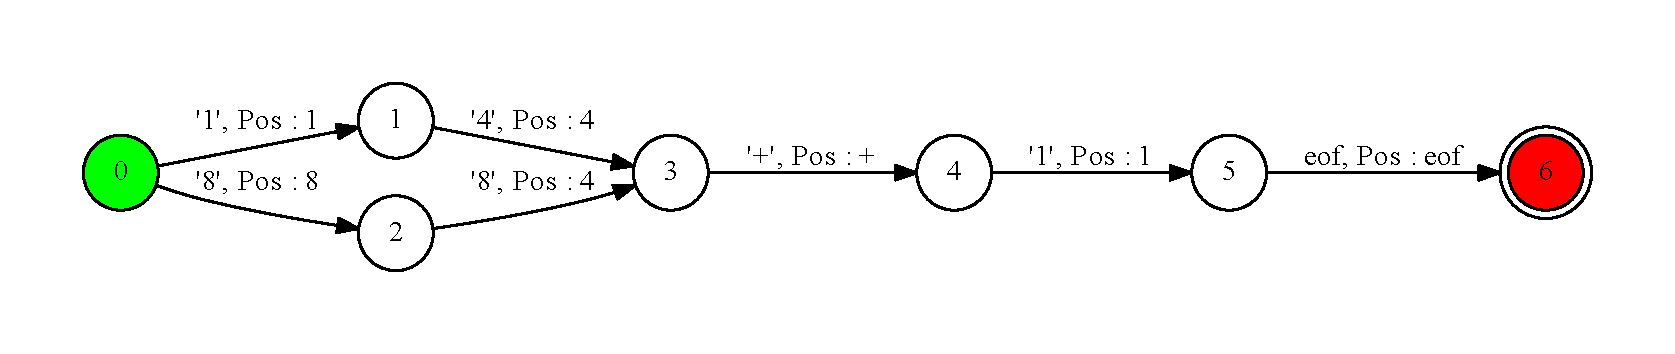
\includegraphics[width=\linewidth]{Gumin/pictures/example_.pdf}
        \caption{Конечный преобразователь $T_1$}
        \label{compose1} 
\end{figure}

\begin{figure}[h!]
        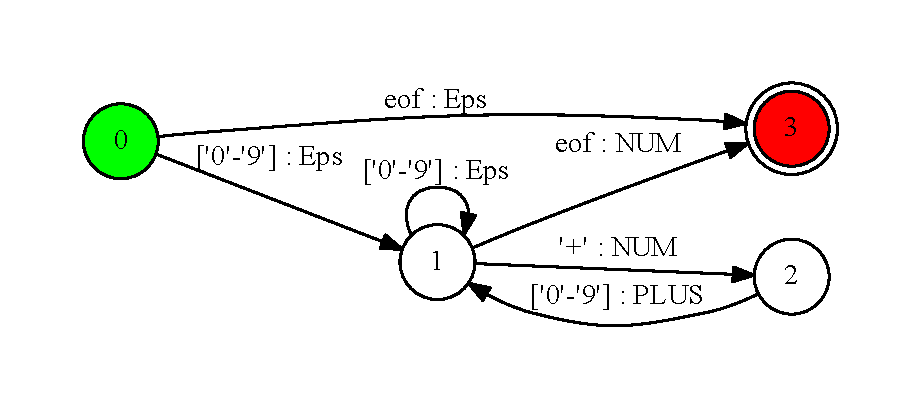
\includegraphics[width=\textwidth]{Gumin/pictures/lexer_.pdf}
        \caption{Конечный преобразователь $T_2$}
        \label{compose2} 
\end{figure}

\begin{figure}[h!]
        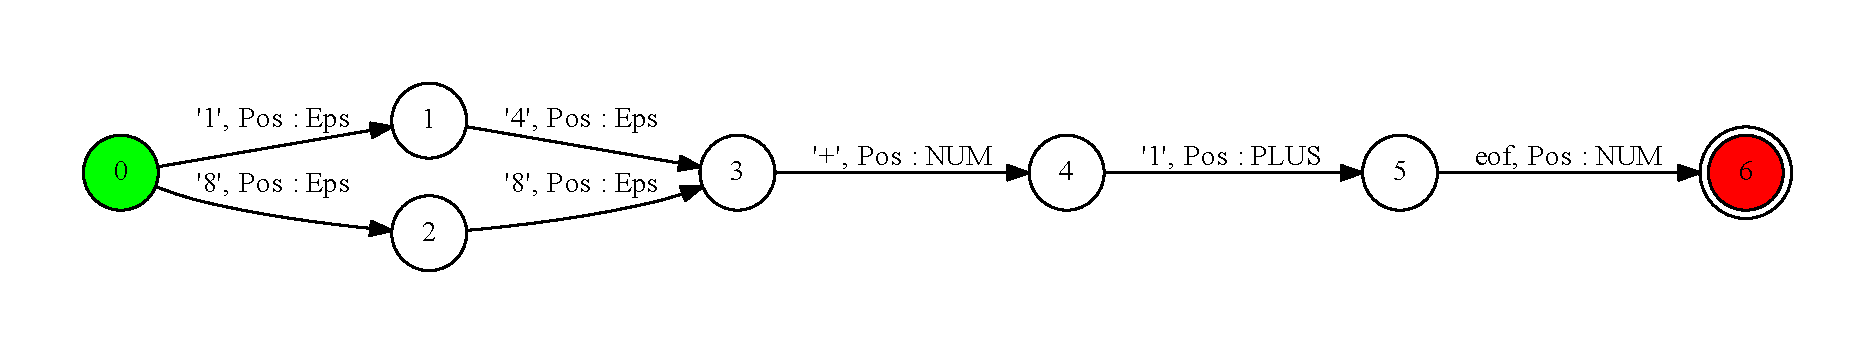
\includegraphics[width=\linewidth]{Gumin/pictures/res_.pdf}
        \caption{Результат композиции конечных преобразователей $T_1$ и $T_2$}
        \label{compose3} 
\end{figure}

\subsection{Символьные конечные преобразователи}
При разработке лексических анализаторов часто возникает ситуация, когда из одного состояния в другое необходимы переходы сразу по нескольким символам. Преобразователи часто реализовывают как некоторые графы, и каждый переход представляется как дуга в этом графе. Соответственно, при разработке лексических анализаторов часто приходится добавлять много дублирующих ребер, например, если необходимо по любой цифре перейти из состояния $A$ в состояние $B$, нужно добавить 10 дуг (рис.~\ref{fig:numfst}). Чем больше ребер в графе, тем больше расход памяти и ниже производительность.

Для борьбы с этой проблемой был предложен символьный конечный преобразователь (Symbolic Transducer)~--- конечный преобразователь,  каждому переходу которого можно сопоставить не один символ, а формулу (например, регулярное выражение). Таким образом, в приведенном выше примере вместо десяти дуг будет одна дуга, которой соответствует регулярное выражение (рис.~\ref{fig:numst}), описывающее цифры. Такие преобразователи получаются гораздо более компактными. 

\begin{figure}[h!]
    \begin{center}
        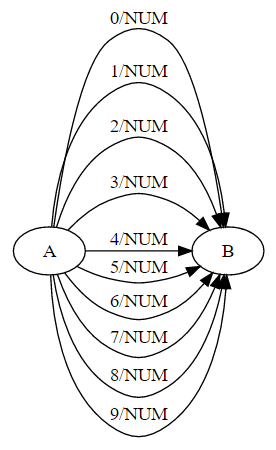
\includegraphics[width=\linewidth/3]{Gumin/pictures/NumFST.png}
        \caption{Пример конечного преобразователя}
        \label{fig:numfst} 
    \end{center}
\end{figure}

\begin{figure}[h!]
    \begin{center}
        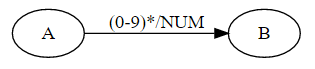
\includegraphics[width=\linewidth/2]{Gumin/pictures/NumST.png}
        \caption{Символьный конечный преобразователь, эквивалентный конечному преобразователю на рис. 4}
        \label{fig:numst} 
    \end{center}
\end{figure}

\textbf{Символьный конечный преобразователь} можно задать шестеркой элементов: 
$\langle Q, \Sigma, \Delta, q_0, F, E \rangle$, где

\begin{itemize}
\item $Q$~--- множество состояний, 
\item $\Sigma$~--- входной алфавит, 
\item $\Delta$~--- выходной алфавит, 
\item $q_0 \in Q$~--- начальное состояние, 
\item $F \subseteq Q$~--- набор конечных состояний, 
\item $E \subseteq Q \times (R(\Sigma) \cup \{\varepsilon\}) \times (\Delta \cup \{\varepsilon\})  \times Q$~--- набор переходов, $R(X)$~--- некоторая формула (в нашем случае~--- регулярное выражение) над множеством $X$.
\end{itemize}

\subsection{Лексический анализ}
Основной задачей лексического анализа является выделение лексем во входном потоке с сохранением их привязки к исходному коду. При классическом лексическом анализе поток символов линеен, но в случае анализа встроенного кода он является нелинейным. Поэтому применяется следующий подход:

\begin{enumerate}
\item В некоторой точке программы по множеству значений строкового выражения строится конечный автомат $M$, аппроксимирующий его сверху.
\item По автомату $M$ строится конечный преобразователь.
\item Производится композиция конечного преобразователя $M'$ с конечным преобразователем, являющимся лексическим анализатором языка, на котором написано выражение.
\item По результирующему преобразователю строится конечный автомат над лексемами, который и является токенизированным входом.
\end{enumerate}

Сложность операции композиции зависит от количества ребер, символьные преобразователи обычно содержат меньшее их количество, чем эквивалентные конечные преобразователи, что позволяет увеличить производительность композиции.

\subsection{Библиотека Microsoft.Automata}
Microsoft.Automata~--- .NET-библиотека, содержащая реализации конечных автоматов, конечных преобразователей, операции над ними и средства их анализа. Библиотека состоит из следующих модулей.
\begin{itemize}
\item Automata~--- основной модуль с реализацией автоматов и преобразователей, содержащий в себе такие элементы, как:
    \begin{itemize}
    \item синтаксические анализаторы грамматик для построения по ним автоматов;
    \item синтаксические анализаторы регулярных выражений, используемых при построении преобразователей;
    \item различные структуры данных, например, BDD;
    \item символьные автоматы и операции над ними;
    \item символьные преобразователи и операции над ними~\cite{STcompose}. 
    \end{itemize}
\item Automata.Z3~--- модуль, обеспечивающий интеграцию реализованных формализмов с SMT-решателем Z3~\cite{Z3Url, articleZ3}.
\item Bek~--- модуль, позволяющий работать с преобразователями и автоматами, используя язык Bek Z3~\cite{BekUrl, BekArticle}. Язык Bek~--- предметно-ориентированный язык для написания и анализа конечных преобразователей, работающих со строками, который является аналогом регулярных выражений для автоматов. Программы на Bek позволяют ответить на вопросы <<выводят ли две программы одну и ту же строку>>, <<может ли эта программа вывести некоторую строку?>>, <<что будет, если выполнить композицию программ?>>.

На листинге~\ref{lst1} приведен пример программы на языке Bek. Программа проходит по строке, используя переменную c, чтобы итерироваться по символам и булеву переменную b, чтобы отслеживать, был ли предыдущий символ экранирующим и добавляет экранирующий символ перед одинарными или двойными кавычками, если он пропущен. 

\fvset{frame=lines,framesep=5pt}
\begin{listing}[H]
    \begin{pyglist}[language=csharp,numbers=left,numbersep=5pt]
program sanitize(t);
    string s; 
    s := iter(c in t){b := false;}{
            case (!(b) && ((c == '\'') || (c == '\"'))) :
                b := false;
                yield ('\\');
                yield (c);
            case (c == '\\') :
                b := !(b);
                yield (c);
            case (true) :
                b := false;
                yield (c);
            };
    return s;
    \end{pyglist}
\caption{Пример программы на языке Bek}
\label{lst1}
\end{listing}
\end{itemize}
